%Exercise 8.1 prob 47
\documentclass{article}
\usepackage{tikz}
\usepackage{tkz-euclide} % loads  TikZ and tkz-base
%\usetkzobj{all}
\usetikzlibrary{calc,math}

\begin{document}
\begin{figure}[!ht]
	\begin{center}
%Exercise 8.1 prob 47
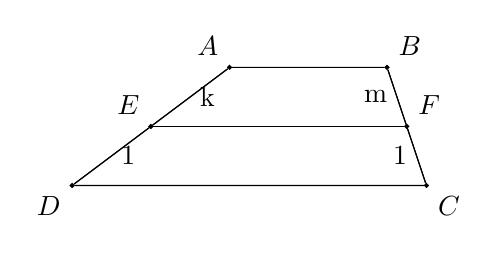
\begin{tikzpicture}
[scale=0.5,>=stealth,point/.style={draw,circle,fill = black,inner sep=0.5pt},]
%\tikzset{shift={(-3,0)}}
%Triangle sides
\def\a{4}
\def\c{9}
\def\xA{4}
\def\h{3}
\def\k{1}
%\def\c{7.5}
\def\yE{\h/2}
%Labeling points
\node (D) at (0,0)[point,label=below left:$D$] {};
\node (B) at ({\xA+\a}, \h )[point,label=above right:$B$] {};
\node (C) at (\c, 0)[point,label=below right:$C$] {};
%\node (E) at (2, \yE)
%\node (F) at (8.5, \yE)[point,label=below right:$F$] {};
%\node (M) at (\xA,\yE)[point,label=above right:$M$] {};
%\node (N) at ({\xA+\a}, \yE)[point,label=above left:$N$] {};
%\node (X) at (\xA , 0)[point,label=below left:$X$] {};
%\node (Y) at ({\xA+\a}, 0)[point,label=below right:$Y$] {};
\node (A) at (\xA , \h)[point,label=above left:$A$] {};
\node (E) at ($(D)!0.5!(A)$)[point,label=above left:$E$] {};
\node (F) at ($(B)!0.5!(C)$)[point,label=above right:$F$] {};



%A



%Drawing parallelogram ABCD
\draw (A) -- (B)--(C) --(D)--(A);
%\draw (A) --(X);
\draw (E) --(F);
\draw(A)--node[right]{$\textrm{k}$} (E)--node[right]{$\textrm{1}$} (D);
\draw(B)--node[left]{$\textrm{m}$} (F)--node[left]{$\textrm{1}$} (C);


%\draw (B) --(Y);
%marking right angles
%\tkzMarkRightAngle[fill=green!20,size=.2](D,X,A)
%\tkzMarkRightAngle[fill=green!20,size=.2](C,Y,B)


%
\end{tikzpicture}
	\end{center}
\caption{Trapezium ABCD}
\label{fig:trapezium_ABCD}	
\end{figure}
\end{document}
